    \documentclass{llncs}

\usepackage[utf8]{inputenc}
\usepackage{amsmath}
\usepackage{graphicx}
\usepackage{amsfonts}
\usepackage{amssymb}
\usepackage{url}
\usepackage{float}
\usepackage{setspace}
\onehalfspacing

\begin{document}

% \let\thefootnote\relax\footnotetext{Copyright \textcopyright  2021 for this paper by its authors. Use permitted under Creative Commons License Attribution 4.0 International (CC BY 4.0). \conference{CLEF 2021 -- Conference and Labs of the Evaluation Forum, September 21--24, 2021, Bucharest, Romania}}


\title{Multi Regressor Based User Rating Predictor (ImageCLEF Aware)}


\author{ Aarthi Suresh Kumar\inst{1}, Anirudh A\inst{2}, Jeet Golecha M\inst{3}, Karthik Raja A\inst{4} \and Bhuvana Jayaraman \inst{5} \and Mirnalinee T T \inst{6}}
\institute{
SSN College of Engineering, India\\
\url{(aarthi19003, anirudh19015,jeetgolecha19043, karthikraja19048, bhuvanaj, mirnalineett)@cse.ssn.edu.in}
}


\maketitle
\begin{abstract}
Every one of the public nowadays have their presence in social media networks.  The profile information of the social media account helps to understand nature of  the user. Images, that  are part of the profile information mostly characterizes  the user and reveals much more about the user than the textual information. Such information extracted are used in many applications namely the  employers, credit scoring, etc.\cite{li2017neural}



Analysis of images is a vitally important task in any field of domain.
Images constitute a large part of the content shared on social networks. Their disclosure is often related to a particular context and users are often unaware of the fact that, depending on their privacy status, images can be accessible to third parties and be used for purposes which were initially unforeseen.
\keywords{{Multi Output Regressor}, {Random Forest}, {Extra Trees}, {Neural Network}, {Scikit Tree}, {User Rating}}

\end{abstract}

\section{Introduction}  
According to a recent report, people are uploading data online at the rate of 1.8 billion images per day.  This statistic adds up to around 657 billion photos\cite{nguyen2022unveiling} every year \cite{photoNum}. Most of these image files are in social networking platforms which can be accessed publicly. However, the owners of these digital images are often unaware of the fact that third parties could access them for a plethora of unethical reasons. Examples include the practice of obtaining information of potential employees by employers and using a user's online data to obtain an automatic credit score. 

Existing methods  rate the information a user uploads online. For instance, Bargh et. al. \cite{barghFeedbackSystem} explored the implications of public user data in the area of user privacy. The paper outlined how user data could be used to derive sensitive information about a user. It also introduced a feedback system from the data recipients to the data disseminators to curb the issue of leaking private information. Other similar approaches focus on inferring user characteristics and their practical utility is rather limited. 
\\This paper aims to develop a more data-centric approach to solving the problem of online user data scoring. It explores the efficacy of two classes of models, namely, regression models and deep learning models to predict the pertinence of a user's data to the following situations:
\begin{enumerate}
    \item Bank Loan
    \item Accommodation 
    \item Applying to a job as a waitress/waiter
    \item Applying to a job in IT
\end{enumerate} 
The regression based models include the Random Forest Regressor, Extra Trees Regressor and the Mutli-Output Regressor. A dense neural network was the deep learning model used for the user data feedback system. Of these models, the Random Forest Regressor performed the best, with a validation error of 0.49. The regression class on models performed better than the deep learning model.

\vspace{5mm}

\section{Task and Dataset}
ImageCLEFAware 2022 deals with developing models to predict the user ratings\cite{hsu2014predicting} for 4 distinct situations given the scores of different visual concepts. The models are expected to provide rankings for user test profiles that are as close as possible to the human rankings.

A data set of 1000 user profiles with 100 photos per profile was created and annotated with an appeal score for a series of real-life situations via crowdsourcing. A global rating\cite{armstrong1995movie} was provided for each profile in each situation modeled using a 7-points Likert scale ranging from strongly unappealing to strongly appealing. An averaged and normalized appeal score was used to create a ground truth composed of ranked users in each modeled situation. Prediction files, which contain visual concepts associated with each user, constitute the training data.  Gt\_files, which contain the the appeal score for each user for each real-life situation. A file with the score for each visual concept was provided as well. Incorporating the scores of each visual concept did not change the result.

\section{Methodologies}
\subsection{Data Preprocessing} 
Prior to applying the machine learning and deep learning techniques, some preprocessing techniques were applied. The location of the visual concepts and the scores for each real-life situation were concatenated and made into a stacked matrix for each user. The cases involved not adding some of this features to reduce diverging, but all patterns gave similar results on accuracy.

\subsection{Regression Models}
\label{Model1Architecture}

\begin{figure}[h]
    \centering
    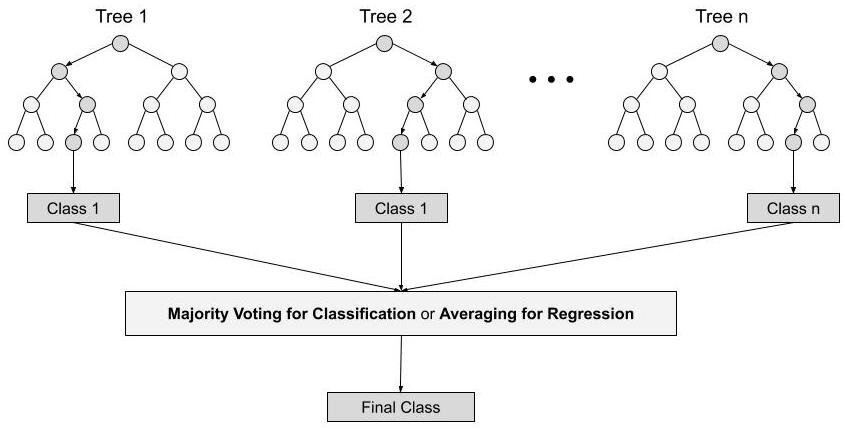
\includegraphics[width=\textwidth,height=\textheight,keepaspectratio]{Random_forest.jpg}
    \caption{Random Forest}
    \label{fig:Model}
\end{figure}


\subsubsection{Random Forest Regressor}
\hfill\\Random forests or random decision forests is an ensemble learning method for classification, regression and other tasks that operates by constructing a multitude of decision trees at training time. For classification tasks, the output of the random forest is the class selected by most trees. A Random Forest\cite{ajesh2016random} is an ensemble of decision trees. This is to say that many trees, constructed in a certain “random” way form a Random Forest. 

Each tree is created from a different sample of rows and at each node, a different sample of features is selected for splitting.  Each of the trees makes its own individual prediction. These predictions combined to produce a single result. The most common methods for the same include majority voting for classification tasks and averaging for regression tasks.

\subsubsection{Extra Trees Regressor}
\hfill\\ Extra Trees is an ensemble machine learning algorithm that combines the predictions from many decision trees. It is a commonly used random forest algorithm. Although it uses a simpler approach to create the decision trees used as members of the ensemble, it can often yield similar or better results than the random forest algorithm.

Both the Random Forest Regressor and the Extra Trees Regressor are tree algorithms. The difference is that the Random Forest Regressor uses resampling and the Extra Trees Regressor uses original data to create the random forest of decision trees.

\subsubsection{Multi Output Regressor}
\hfill\\ The two models discussed above output only a single real value. Hence, they are modified to produce multiple outputs using the Multi Output Regressor(MOR) function. The MOR function runs the Random Forest and Extra Tree Regresors 4 times to get the values for each of the real-life situations. 
\subsection{Deep Learning Model}
A dense neural network was also explored. A dense neural network consists of dense layers. A dense layer is one that is connected to every neuron of its preceding layer. The dense neural network used for this task consists of 7 dense layers. The input is flattened into a 3000 point vector before passing it into the first layer of the dense neural network. The output of the dense neural network is a 4-point vector. The architecture of the deep learning model is shown below.
\begin{figure}[h]
    \centering
    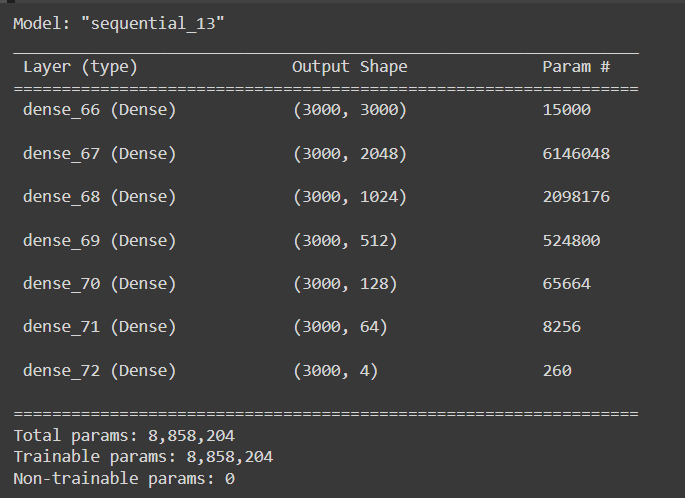
\includegraphics[width=\textwidth,height=\textheight,keepaspectratio]{DL_model.png}
    \caption{Deep Learning Model}
    \label{fig:Randomforest}
\end{figure}

\newpage
\subsection{Training and Validation Set}
In this section, we present a concise anaylsis of the two best models: Random Forest Regressor and Extra Trees Regressor. The training accuracy of the former was less than the latter. This can be attributed to the fact that the Random Forest Regressor uses the concept of bootstrap re-sampling, bringing in new data that can diverge from actual data for training. 

On the other hand, the validation accuracy of the Random Forest Regressor was better than that of the Extra Trees regressor by approximately 0.01\%.

\section{Tested Models}
The regression and deep learning models were tested. The regression class of models performed better than the deep learning model. The 7 layer dense neural network had a validation accuracy of 0.15. It followed the same preprocessing techniques as the regression models. We suspect that lack of data can attributed to this poor accuracy. Hence, we had to alter our model to a much simpler neural network that can work with smaller amount of data. 


\section{Hardware used}
A Google Colab notebook was used to train the model. A general purpose RAM 
size of 8GB was alloted with a 2.3GHz Intel Xenon CPU.


\section {Code}
The resources used by JBTTM for CLEF aware, including the research papers, exploratory data analysis, and code can be found here: \url{https://github.com/AAnirudh07/CLEF-2022}

\section{Result}
The Pearson Correlation Coefficient is a measure of linear correlation between two sets of data. The formula is provided below.
\begin{figure}[h]
    \centering
    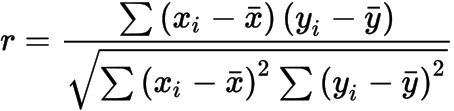
\includegraphics[width=0.5\textwidth,height=0.5\textheight,keepaspectratio]{correlation_coefficient_formula.png}
    \caption{Pearson Correlation Coefficient}
    \label{fig:Randomforest}
\end{figure}
\hfill\\ Team JBTTM had a maximum observed Pearson Correlation Coefficient of 0.139. It was the Random Forest Regressor that had this value.  

\section{Conclusion}
Of the 3 submissions that team JBTTM made, the regression model had the best accuracy based on the metrics proposed by CLEF. The accuracy of the 7 layer deep learning model was inferior to the machine learning models and, no further improvements were made to it. In conclusion, machine learning models are more suitable for the task of user data rating than deep learning models. These results may also be attributed to the lack of training data.

\bibliographystyle{splncs}

%
\bibliography{references}

%
\end{document}